%!TEX root=../../main.tex


%_______________
\section{Exercises}

\noindent

%_______________
\subsection{Case study: preventing peanut allergies}

% 1

\eoce{\qt{Migraine and acupuncture\label{migraine_and_acupuncture_intro}} Acupuncture is sometimes recommended as a treatment option for migraines; a migraine is a particularly painful type of headache. To determine whether acupuncture relieves migraine 
	pain, researchers conducted a randomized controlled study in which 89 females 
	diagnosed with migraines were randomly assigned to one of two groups: 
	treatment or control. The 43 patients in the treatment group received acupuncture 
	that is specifically designed to treat migraines, while 46 patients in the control 
	group received placebo acupuncture (needle insertion at a non-acupoint 
	locations). 24 hours after receiving acupuncture, patients were asked 
	if they were pain free; the results are summarized in the contingency table below. 
	\footfullcite{Allais:2011}
	
	\noindent\begin{minipage}[l]{0.4\textwidth}
		\begin{tabular}{ll  cc c} 
			&           & \multicolumn{2}{c}{\textit{Pain free}} \\
			\cline{3-4}
			&			 & Yes 	    & No 	                      & Total	\\
			\cline{2-5}
			& Treatment & 10	 	& 33		                  & 43 	\\
			\raisebox{1.5ex}[0pt]{\emph{Group}}  & Control	 & 2	 	& 44 	 	                  & 46 \\
			\cline{2-5}
			&Total		 & 12		& 77		                  & 89
		\end{tabular}
	\end{minipage}
	\begin{minipage}[c]{0.05\textwidth}
	\end{minipage}
	\begin{minipage}[c]{0.27\textwidth}
		\begin{center}
			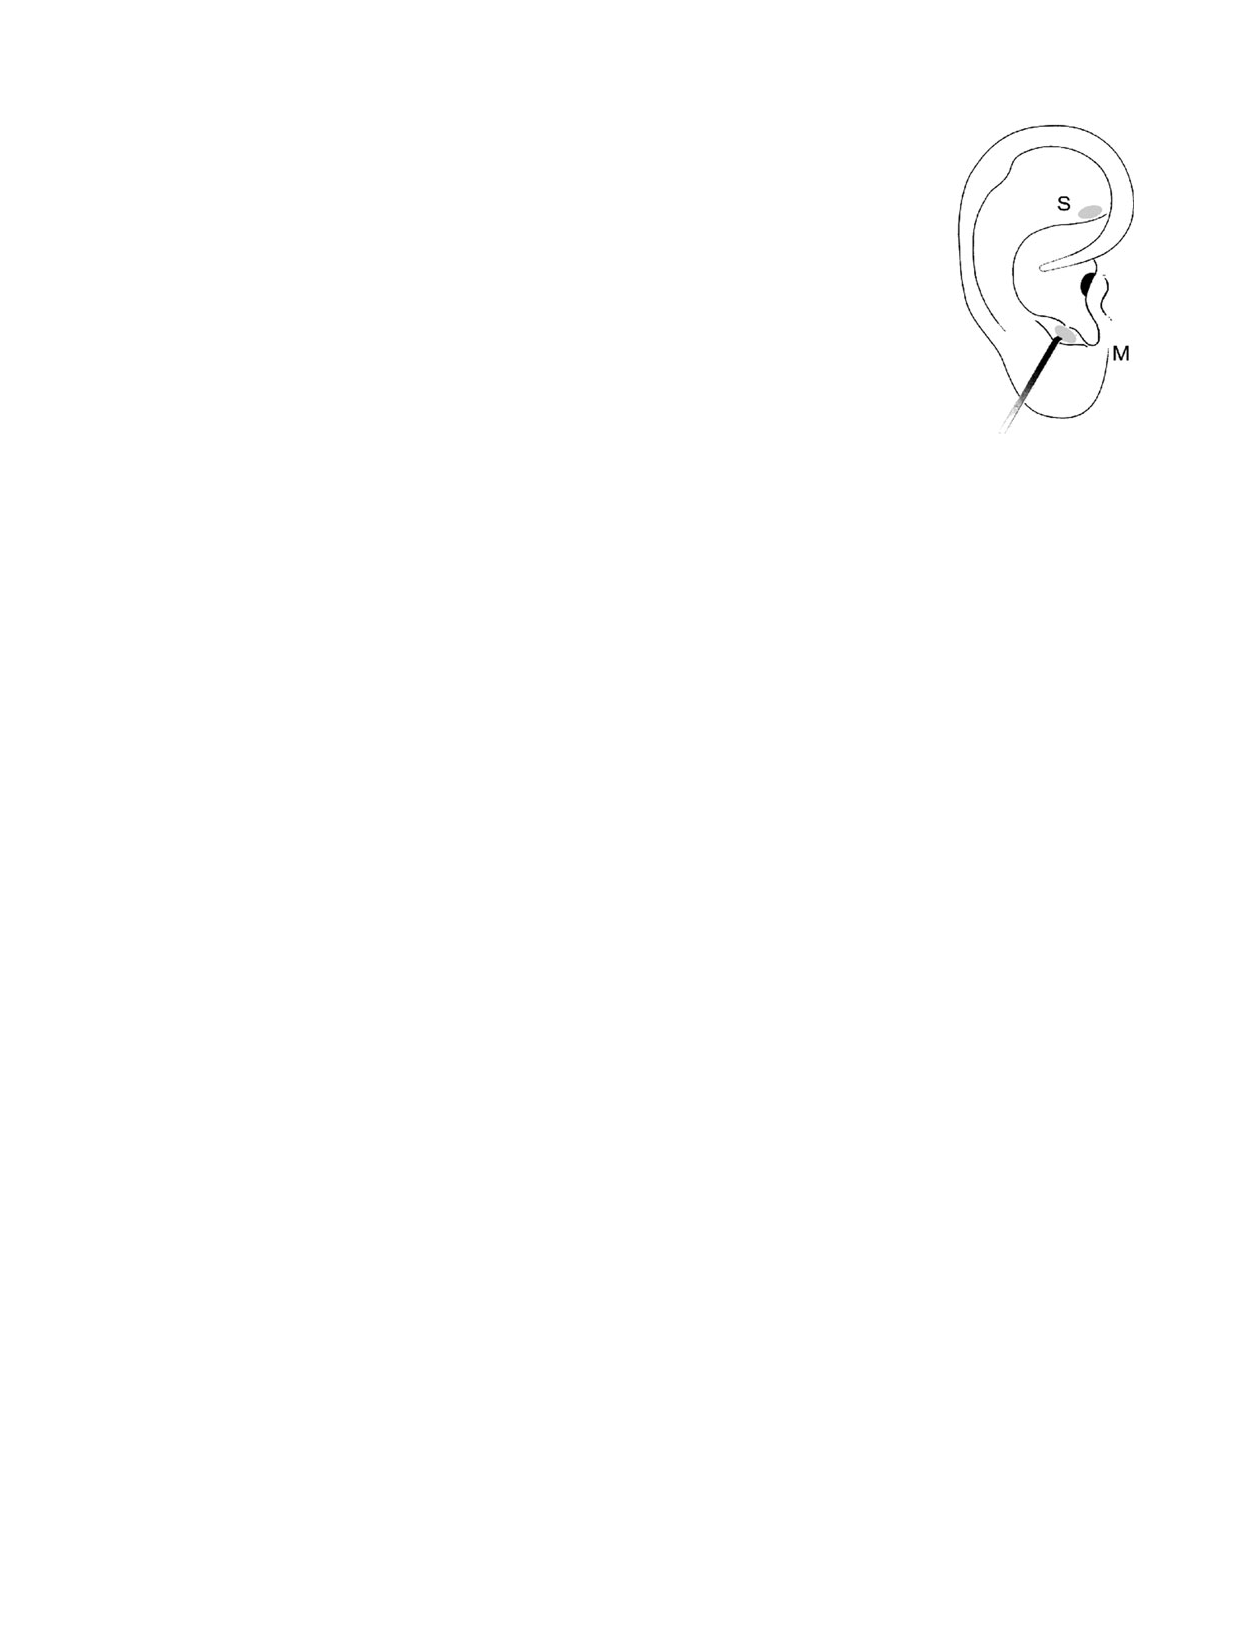
\includegraphics[width = 0.75\textwidth]{ch_intro_to_data_oi_biostat/figures/eoce/migraine_and_acupuncture_intro/earacupuncture.pdf}
		\end{center}
	\end{minipage}
	\begin{minipage}[c]{0.25\textwidth}
		{\footnotesize Figure from the original paper displaying the appropriate area 
			(M) versus the inappropriate area (S) used in the treatment of migraine attacks.}
	\end{minipage}
	
	\begin{parts}
		\item What percent of patients in the treatment group were pain free 24 hours 
		after receiving acupuncture? What percent in the control group?
		\item At first glance, does acupuncture appear to be an effective treatment for 
		migraines? Explain your reasoning.
	\end{parts}
}{}


% 2

\eoce{\qt{Sinusitis and antibiotics\label{sinusitis_and_antibiotics_intro}} 
	Researchers studying the effect of antibiotic treatment for acute sinusitis randomly assigned 166 adults diagnosed with acute sinusitis to either the treatment or control group. Patients in the treatment group received a 10-day course of amoxicillin, while patients in the control group received a placebo consisting of symptomatic treatments, such as nasal decongestants. At the end of the 10-day period, patients were asked if they experienced significant improvement in their symptoms. The distribution of responses are summarized below. 
	\footfullcite{Garbutt:2012}
	\begin{center}
		\begin{tabular}{ll  cc c} 
			&			& \multicolumn{2}{c}{\textit{Self-reported significant}} \\
			&			& \multicolumn{2}{c}{\textit{improvement in symptoms}} \\
			\cline{3-4}
			&			& Yes 	& No 	& Total	\\
			\cline{2-5}
			& Treatment & 66	& 19	& 85 \\
			\raisebox{1.5ex}[0pt]{\emph{Group}}	& Control	& 65	& 16 	& 81 \\
			\cline{2-5}
			& Total		& 131	& 35	& 166
		\end{tabular}
	\end{center}
	\begin{parts}
		\item What percent of patients in the treatment group experienced a significant 
		improvement in symptoms? What percent in the control group?
		\item Based on your findings in part (a), which treatment appears to be more 
		effective for sinusitis?
		\item Does it seem like the observed difference could just be due to chance?
	\end{parts}
}{}


%_______________
\subsection{Data basics}

% 3

\eoce{\qt{Air pollution and birth outcomes, study components\label{study_components_airpoll}} 
Researchers collected data to examine the relationship between air pollutants 
and preterm births in Southern California. During the study, air pollution levels 
were measured by air quality monitoring stations. Specifically, levels of carbon 
monoxide were recorded in parts per million, nitrogen dioxide and ozone in parts 
per hundred million, and coarse particulate matter (PM$_{10}$) in $\mu g/m^3$. 
Length of gestation data were collected for 143,196 births between the years 1989 
and 1993, and air pollution exposure during gestation was calculated for each 
birth. The analysis suggested that increased ambient PM$_{10}$ and, to a lesser 
degree, CO concentrations may be associated with the occurrence of preterm births. 
\footfullcite{Ritz+Yu+Chapa+Fruin:2000} Identify \begin{inparaenum}[(a)]
	\item the cases,
	\item the variables and their types, and
	\item the main research question
\end{inparaenum} 
	in this study.
}{}

% 4

\eoce{\qt{Buteyko method, study components\label{study_components_buteyko}} 
The Buteyko method is a shallow breathing technique developed by Konstantin 
Buteyko, a Russian doctor, in 1952. Anecdotal evidence suggests that the Buteyko 
method can reduce asthma symptoms and improve quality of life. In a scientific 
study to determine the effectiveness of this method, researchers recruited 600 
asthma patients aged 18-69 who relied on medication for asthma treatment. These 
patients were split into two research groups: one practiced the Buteyko method 
and the other did not. Afterwards, patients were scored on quality of life, activity, 
asthma symptoms, and medication reduction on a scale from 0 to 10. On average, 
the participants in the Buteyko group experienced a significant reduction in 
asthma symptoms and an improvement in quality of life. \footfullcite{McDowan:2003} 
Identify \begin{inparaenum}[(a)]
\item the cases,
\item the variables and their types, and
\item the main research question 
\end{inparaenum}
in this study.
}{}

% 5 (oi_biostat)

\eoce{\qt{Hummingbird taste behavior, study components\label{study_components_hummingbirds}}
Researchers hypothesized that a particular taste receptor in hummingbirds, T1R1-T1R3, played a primary role in dictating taste behavior; specifically, in determining which compounds hummingbirds detect as sweet. In a series of field tests, hummingbirds were presented simultaneously with two filled containers, one containing test stimuli and a second containing sucrose. The test stimuli included aspartame, erythritol, water, and sucrose. Aspartame is an artificial sweetener that tastes sweet to humans, but is not detected by hummingbird T1R1-T1R3 , while erythritol is an artificial sweetener known to activate T1R1-T1R3.

Data were collected on how long a hummingbird drank from a particular container for a given trial, measured in seconds. For example, in one field test comparing aspartame and sucrose, a hummingbird drank from the aspartame container for 0.54 seconds and from the sucrose container for 3.21 seconds. 
\begin{parts}
\item Which tests are controls? Which tests are treatments?
\item Identify the response variable(s) in the study. Are they numerical or categorical?
\item Describe the main research question.
\end{parts}	
}{}

%citation: hummingbirds, pset 5

% 6 (oi_biostat)

\eoce{\qt{Egg coloration\label{egg_coloration}}
The evolutionary significance of variation in egg coloration among birds is not fully understood. One hypothesis suggests that egg coloration may be an indication of female quality, with healthier females being capable of depositing blue-green pigment into eggshells instead of using it for themselves as an antioxidant. In a study conducted on 32 collared flycatchers, half of the females were given supplementary diets before and during egg laying. Eggs were measured for darkness of blue color using spectrophotometry; for example, the mean amount of blue-green chroma was 0.594 absorbance units. Egg mass was also recorded.
\begin{parts}
\item Identify the control and treatment groups.
\item Describe the main research question.
\item Identify the primary response variable of interest, and whether it is numerical or categorical.
\end{parts}
}{}

%citation: blue_eggs_food

% 7

\eoce{\qt{Smoking habits of UK residents\label{smoking_habits_UK_datamatrix}} A survey 
was conducted to study the smoking habits of UK residents. Below is a data 
matrix displaying a portion of the data collected in this survey. Note that 
``$\pounds$" stands for British Pounds Sterling, ``cig" stands for cigarettes, 
and ``N/A'' refers to a missing component of the data. \footfullcite{data:smoking}
\begin{center}
\scriptsize{
\begin{tabular}{rccccccc}
\hline
	& sex 	 & age 	& marital 	& grossIncome 					     & smoke & amtWeekends	& amtWeekdays \\ 
\hline
1 	& Female & 42 	& Single 	& Under $\pounds$2,600 			     & Yes 	 & 12 cig/day   & 12 cig/day \\ 
2 	& Male	 & 44	& Single 	& $\pounds$10,400 to $\pounds$15,600 & No	 & N/A 			& N/A \\ 
3 	& Male 	 & 53 	& Married   & Above $\pounds$36,400 		     & Yes 	 & 6 cig/day 	& 6 cig/day \\ 
\vdots & \vdots & \vdots & \vdots & \vdots 				             & \vdots & \vdots 	    & \vdots \\ 
1691 & Male  & 40   & Single 	& $\pounds$2,600 to $\pounds$5,200   & Yes 	 & 8 cig/day 	& 8 cig/day \\   
\hline
\end{tabular}
}
\end{center}
\begin{parts}
\item What does each row of the data matrix represent?
\item How many participants were included in the survey?
\item For each variable, indicate whether it is numerical or categorical. If numerical, identify the variable as continuous or discrete. If categorical, indicate if the variable is ordinal.
\end{parts}
}{}

% 8 (oi_biostat)

\eoce{\qt{The microbiome and colon cancer\label{microbiome_colon}}
A study was conducted to assess whether the abundance of particular bacterial species in the gastrointestinal system is associated with the development of colon cancer. The following data matrix shows a subset of the data collected in the study. Cancer stage is coded 1-4, with larger values indicating cancer that is more difficult to treat. The abundance levels are given for five bacterial species; abundance is calculated as the frequency of that species divided by the total number of bacteria from all species.
	
\begin{center}	
% latex table generated in R 3.2.4 by xtable 1.8-2 package
% Mon May 30 17:00:41 2016
\begin{table}[ht]
	\centering
\scriptsize{
	\begin{tabular}{rcccccccc}
		\hline
		& age & gender & stage & bug 1 & bug 2 & bug 3 & bug 4 & bug 5 \\ 
		\hline
		1 &  71 & Female &   2 & 0.03 & 0.09 & 0.52 & 0.00 & 0.00 \\ 
		2 &  53 & Female &   4 & 0.16 & 0.08 & 0.08 & 0.00 & 0.00 \\ 
		3 &  55 & Female &   2 & 0.00 & 0.01 & 0.31 & 0.00 & 0.00 \\ 
		4 &  44 & Male &   2 & 0.11 & 0.14 & 0.00 & 0.07 & 0.05 \\ 
		\vdots & \vdots & \vdots & \vdots & \vdots & \vdots & \vdots & \vdots & \vdots \\
		73 &  48 & Female &   3 & 0.21 & 0.05 & 0.00 & 0.00 & 0.04 \\ 
		\hline
	\end{tabular}
}
\end{table}
\end{center}

\begin{parts}
\item What does each row of the data matrix represent?
\item Identify explanatory and response variables.
\item For each variable, indicate whether it is numerical or categorical. 	
\end{parts}
}{}


%_______________
\subsection{Data collection principles}

% 9

\eoce{\qt{Air pollution and birth outcomes, scope of inference\label{scope_airpoll}} 
Exercise~\ref{study_components_airpoll} introduces a study where researchers 
collected data to examine the relationship between air pollutants and preterm 
births in Southern California. During the study, air pollution levels were 
measured by air quality monitoring stations. Length of gestation data were 
collected on 143,196 births between the years 1989 and 1993, and air pollution 
exposure during gestation was calculated for each birth. It can be assumed that the 143,196 births are effectively the entire population of births during this time period.
\begin{parts}
\item Identify the population of interest and the sample in this study.
\item Comment on whether or not the results of the study can be generalized to the 
population, and if the findings of the study can be used to establish causal relationships.
\end{parts}
}{}

% 10

\eoce{\qt{Buteyko method, scope of inference\label{scope_buteyko}} 
Exercise~\ref{study_components_buteyko} introduces a study on using the Buteyko 
shallow breathing technique to reduce asthma symptoms and improve quality of life.
As part of this study 600 asthma patients aged 18-69 who relied on medication for 
asthma treatment were recruited and randomly assigned to two groups: one practiced 
the Buteyko method and the other did not. Those in the Buteyko group experienced,
on average, a significant reduction in asthma symptoms and an improvement in quality 
of life.
\begin{parts}
\item Identify the population of interest and the sample in this study.
\item Comment on whether or not the results of the study can be generalized to the 
population, and if the findings of the study can be used to establish causal 
relationships.
\end{parts}
}{}

% 11 (oi_biostat)

\eoce{\qt{Herbal remedies\label{herbal_remedies}}
Echinacea has been widely used as an herbal remedy for the common cold, but previous studies evaluating its efficacy as a remedy have produced conflicting results. In a new study, researchers randomly assigned 437 volunteers to receive either a placebo or echinacea treatment before being infected with rhinovirus. Healthy young adult volunteers were recruited for the study from the University of Virginia community. 
\begin{parts}
\item Identify the population of interest and the sample in this study.
\item Comment on whether or not the results of the study can be generalized to a larger population. 
\item Can the findings of the study be used to establish causal relationships? Justify your answer.
\end{parts} 
}{}

% 12, edited

\eoce{\qt{Vitamin supplements\label{vitamin_supplement}} In order to assess the effectiveness 
	of taking large doses of vitamin C in reducing the duration of the common cold, 
	researchers recruited 400 healthy volunteers from staff and students at a university. A 
	quarter of the patients were randomly assigned a placebo, and the rest were randomly allocated between 1g Vitamin C, 3g Vitamin C, or 3g Vitamin C plus additives to be taken at onset of a cold for the following two days. All tablets had identical appearance and packaging. No significant differences were observed in any measure of cold duration or severity between the four medication groups, and the placebo group had the shortest duration of symptoms.\footfullcite{Audera:2001}
	\begin{parts}
		\item Was this an experiment or an observational study? Why?
		\item What are the explanatory and response variables in this study?
		\item Participants are ultimately able to choose whether or not to use the pills 
		prescribed to them. We might expect that not all of them will adhere and take their 
		pills. Does this introduce a confounding variable to the study? Explain your reasoning.
	\end{parts}
}{}

% 13

\eoce{\qt{Exercise and mental health\label{exercise_mental_health}} A researcher is interested 
	in the effects of exercise on mental health and he proposes the following study: Use 
	stratified random sampling to recruit 18-30, 31-40 and 41-55 year olds from the population. Next, randomly assign half the subjects from each age 
	group to exercise twice a week, and instruct the rest not to exercise. Conduct a mental 
	health exam at the beginning and at the end of the study, and compare the results.
	\begin{parts}
		\item What type of study is this? 
		\item What are the treatment and control groups in this study?
		\item Does this study make use of blocking? If so, what is the blocking variable?
		\item Comment on whether or not the results of the study can be used to establish a 
		causal relationship between exercise and mental health, and indicate whether or not the 
		conclusions can be generalized to the population at large.
		\item Suppose you are given the task of determining if this proposed study should get 
		funding. Would you have any reservations about the study proposal?
	\end{parts}
}{}

% 14 (oi_biostat)

\eoce{\qt{Chicks and antioxidants\label{chicks_antioxidants}}
Environmental factors early in life can have long-lasting effects on an organism. In one study, researchers examined whether dietary supplementation with vitamins C and E influences body mass and corticosterone level in yellow-legged gull chicks. Chicks were randomly assigned to either the nonsupplemented group or the vitamin supplement experimental group. The initial study group consisted of 108 nests, with 3 eggs per nest. Chicks were assessed at age 7 days. 
\begin{parts}
\item What type of study is this?
\item What are the experimental and control treatments in this study?
\item Explain why randomization is an important feature of this experiment.
\end{parts}
}{}

% adapted from chicks_antioxidants

\newpage

% 15

\eoce{\qt{Internet use and life expectancy\label{internet_life_expectancy}} Data were collected to evaluate the relationship between estimated life expectancy at birth (as of 2014) and 
percentage of internet users (as of 2009) in 208 countries for which such 
data were available.\footfullcite{data:ciaFactbook}
\begin{parts}
\item What type of study is this?
\item State a possible confounding variable that might explain this relationship 
and describe its potential effect.
\end{parts}
}{}

% 16

\eoce{\qt{Stressed out\label{stressed_out_observational}} A study that 
surveyed a random sample of otherwise healthy high school students found that 
they are more likely to get muscle cramps when they are stressed. The study 
also noted that students drink more coffee and sleep less when they are 
stressed.
\begin{parts}
\item What type of study is this?
\item Can this study be used to conclude a causal relationship between 
increased stress and muscle cramps?
\item State possible confounding variables that might explain the observed 
relationship between increased stress and muscle cramps. 
\end{parts}
}{}

% 17, context edited

\eoce{\qt{Evaluate sampling methods\label{evaluate_sampling_methods}}
A university wants to assess how many hours of sleep students are getting per night. For each proposed method below, discuss whether the method is reasonable or not.
\begin{parts}
\item Survey a simple random sample of 500 students.
\item Stratify students by their field of study, then sample 10\% of students from each stratum.
\item Cluster students by their class year (e.g. freshmen in one cluster, sophomores in one cluster, etc.), then randomly sample three clusters and survey all students in those clusters.
\end{parts}}{}

% 18

\eoce{\qt{Flawed reasoning\label{flawed_reasoning}} Identify the flaw(s) in reasoning 
in the following scenarios. Explain what the individuals in the study should 
have done differently if they wanted to make such conclusions.
\begin{parts}
\item Students at an elementary school are given a questionnaire that they 
are asked to return after their parents have completed it. One of the questions 
asked is, ``Do you find that your work schedule makes it difficult for you to 
spend time with your kids after school?" Of the parents who replied, 85\% said 
``no". Based on these results, the school officials conclude that a great 
majority of the parents have no difficulty spending time with their kids 
after school.
\item A survey is conducted on a simple random sample of 1,000 women who 
recently gave birth, asking them about whether or not they smoked during 
pregnancy. A follow-up survey asking if the children have respiratory problems 
is conducted 3 years later, however, only 567 of these women are reached at the 
same address. The researcher reports that these 567 women are representative 
of all mothers.
\item An orthopedist administers a questionnaire to 30 of his patients who do 
not have any joint problems and finds that 20 of them regularly go running. 
He concludes that running decreases the risk of joint problems.
\end{parts}
}{}

% 19

\eoce{\qt{City council survey\label{city_council_survey}} A city council has requested a 
household survey be conducted in a suburban area of their city. The area is broken 
into many distinct and unique neighborhoods, some including large homes, some with 
only apartments, and others a diverse mixture of housing structures. Identify the 
sampling methods described below, and comment on whether or not you think they 
would be effective in this setting.
\begin{parts}
\item Randomly sample 50 households from the city.
\item Divide the city into neighborhoods, and sample 20 households from each 
neighborhood.
\item Divide the city into neighborhoods, randomly sample 10 neighborhoods, 
and sample all households from those neighborhoods.
\item Divide the city into neighborhoods, randomly sample 10 neighborhoods, 
and then randomly sample 20 households from those neighborhoods.
\item Sample the 200 households closest to the city council offices.
\end{parts}
}{}

% 20

\eoce{\qt{Reading the paper\label{reading_paper}} Below are excerpts from two 
articles published in the \emph{NY Times}:
\begin{parts}
\item An article titled \emph{Risks: Smokers Found More Prone to Dementia} 
states the following: \footfullcite{news:smokingDementia}
\begin{adjustwidth}{1em}{1em}
{\footnotesize ``Researchers analyzed data from 23,123 health plan members who 
participated in a voluntary exam and health behavior survey from 1978 to 1985, 
when they were 50-60 years old. 23 years later, about 25\% of the group had 
dementia, including 1,136 with Alzheimer's disease and 416 with vascular 
dementia. After adjusting for other factors, the researchers concluded that 
pack-a-day smokers were 37\% more likely than nonsmokers to develop dementia, 
and the risks went up with increased smoking; 44\% for one to two packs a day; 
and twice the risk for more than two packs."}
\end{adjustwidth}
Based on this study, can it be concluded that smoking causes dementia later in 
life? Explain your reasoning.
\item Another article titled \emph{The School Bully Is Sleepy} states the 
following: \footfullcite{news:bullySleep}
\begin{adjustwidth}{1em}{1em}
{\footnotesize ``The University of Michigan study, collected survey data from 
parents on each child's sleep habits and asked both parents and teachers to 
assess behavioral concerns. About a third of the students studied were 
identified by parents or teachers as having problems with disruptive behavior 
or bullying. The researchers found that children who had behavioral issues and 
those who were identified as bullies were twice as likely to have shown 
symptoms of sleep disorders."}
\end{adjustwidth}
A friend of yours who read the article says, ``The study shows that sleep 
disorders lead to bullying in school children." Is this statement justified? 
If not, how best can you describe the conclusion that can be drawn from this 
study?
\end{parts}
}{}

% 21 (oi_biostat)

\eoce{\qt{Alcohol consumption and STIs\label{alcohol_STIs}}
An observational study published last year in \textit{The American Journal of Preventive Medicine} investigated the effects of an increased alcohol sales tax in Maryland on the rates of gonorrhea and chlamydia.\footnote{S. Staras, et al., 2015. Maryland Alcohol Sales Tax and Sexually Transmitted Infections. The American Journal of Preventive Medicine 50: e73-e80.} After a tax increase from 6\% to 9\% in 2011, the statewide gonorrhea rate declined by 24\%, the equivalent of 1,600 cases per year. In a statement to the \textit{New York Times}, the lead author of the paper was quoted saying, "Policy makers should consider raising liquor taxes if they're looking for ways to prevent sexually transmitted infections. In the year and a half following the alcohol tax rise in Maryland, this prevented 2,400 cases of gonorrhea and saved half a million dollars in health care costs." Explain whether the lead author's statement is accurate.
}{}

% add ref to bib

%_______________
\subsection{Numerical data}

% 22

\eoce{\qt{Medians and IQRs} For each part, compare distributions (1) and (2) based on their medians and IQRs. You do not need to calculate these statistics; simply state how the medians and IQRs compare. Make sure to explain your reasoning. 
	\begin{multicols}{2}
		\begin{parts}
			\item (1) 3, 5, 6, 7, 9 \\
			(2) 3, 5, 6, 7, 20
			\item (1) 3, 5, 6, 7, 9 \\
			(2) 3, 5, 8, 7, 9
			\item (1) 1, 2, 3, 4, 5 \\
			(2) 6, 7, 8, 9, 10
			\item (1) 0, 10, 50, 60, 100 \\
			(2) 0, 100, 500, 600, 1000
		\end{parts}
	\end{multicols}
}{}

% 23

\eoce{\qt{Means and SDs} For each part, compare distributions (1) and (2) based on their means and standard deviations. You do not need to calculate these statistics; simply state how the means and the standard deviations compare. Make sure to explain your reasoning. \textit{Hint:} It may be useful to sketch dot plots of the distributions.
\begin{multicols}{2}
\begin{parts}
\item (1) 3, 5, 5, 5, 8, 11, 11, 11, 13 \\
(2) 3, 5, 5, 5, 8, 11, 11, 11, 20 \\
\item (1) -20, 0, 0, 0, 15, 25, 30, 30 \\
(2) -40, 0, 0, 0, 15, 25, 30, 30
\item (1) 0, 2, 4, 6, 8, 10 \\
(2) 20, 22, 24, 26, 28, 30
\item (1) 100, 200, 300, 400, 500 \\
(2) 0, 50, 300, 550, 600
\end{parts}
\end{multicols}
}{}

% 24

\eoce{\qt{Mix-and-match} Describe the distribution in the histograms below and match them to the box plots. \\
\begin{center}
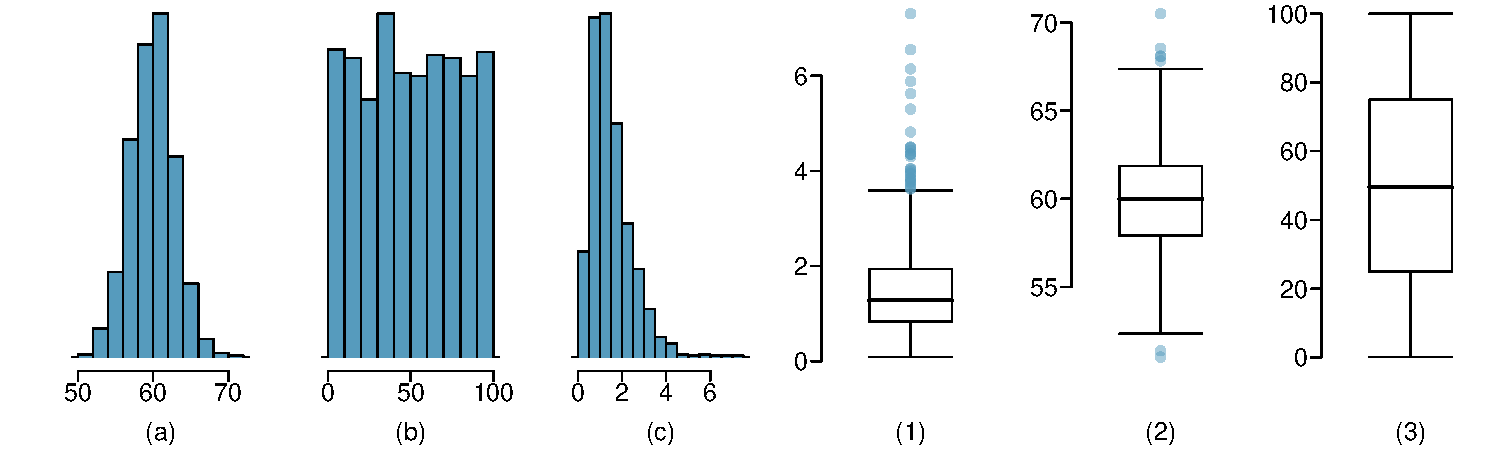
\includegraphics[width=\textwidth]{ch_intro_to_data_oi_biostat/figures/eoce/hist_box_match/hist_box_match.pdf}
\end{center}
}{}

% 25

\eoce{\qt{Air quality\label{air_quality_durham}} Daily air quality is measured by the air 
quality index (AQI) reported by the Environmental Protection Agency. This index reports 
the pollution level and what associated health effects might be a concern. The index is 
calculated for five major air pollutants regulated by the Clean Air Act and takes values 
from 0 to 300, where a higher value indicates lower air quality. AQI was reported for a 
sample of 91 days in 2011 in Durham, NC. The relative frequency histogram below shows 
the distribution of the AQI values on these days. \footfullcite{data:durhamAQI:2011}

\begin{minipage}[c]{0.55\textwidth}
\begin{parts}
\item Based on the histogram, describe the distribution of daily AQI. 
\item Estimate the median AQI value of this sample.
\item Would you expect the mean AQI value of this sample to be higher or lower than the 
median? Explain your reasoning.
\end{parts}
\end{minipage}
\begin{minipage}[c]{0.45\textwidth}
\begin{center}
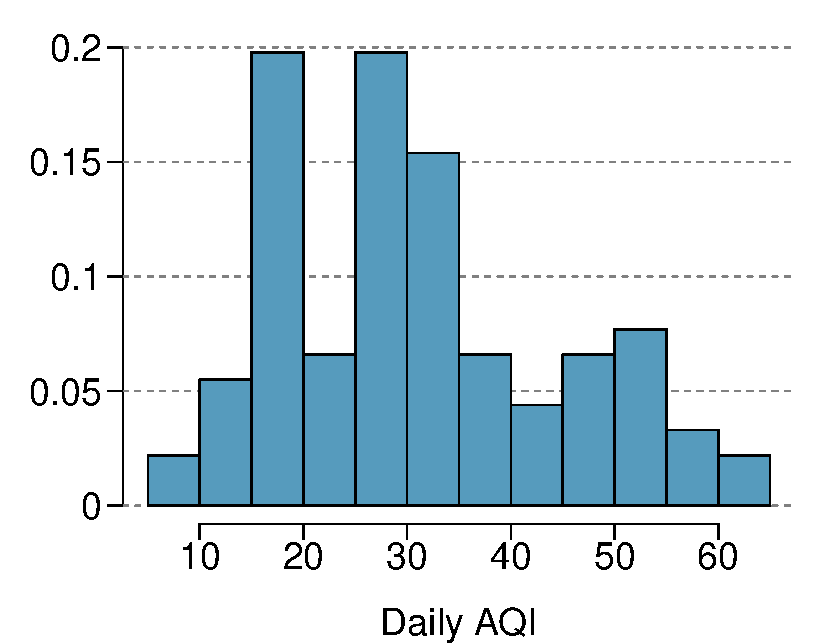
\includegraphics[width = \textwidth]{ch_intro_to_data_oi_biostat/figures/eoce/air_quality_durham/air_quality_durham_rel_freq_hist.pdf} 
\end{center}
\end{minipage}
}{}

% 26 (oi_biostat)

\eoce{\qt{Nursing home residents\label{nursing_homes}}
Since states with larger numbers of elderly residents would naturally have more nursing home residents, the number of nursing home residents in a state is often adjusted for the number of people 65 years of age or order (65+). That adjustment is usually given as the number of nursing home residents age 65+ per 1,000 members of the population age 65+. For example, a hypothetical state with 200 nursing home residents age 65+ and 50,000 people age 65+ would have the same adjusted number of residents as a state with 400 residents and a total age 65+ population of 100,000 residents: 4 residents per 1,000. 

Use the two plots below to answer the following questions. Both plots show the distribution of the number of nursing home residents per 1,000 members of the population 65+ (in each state). 

\begin{minipage}[c]{0.55\textwidth}
\begin{center}
	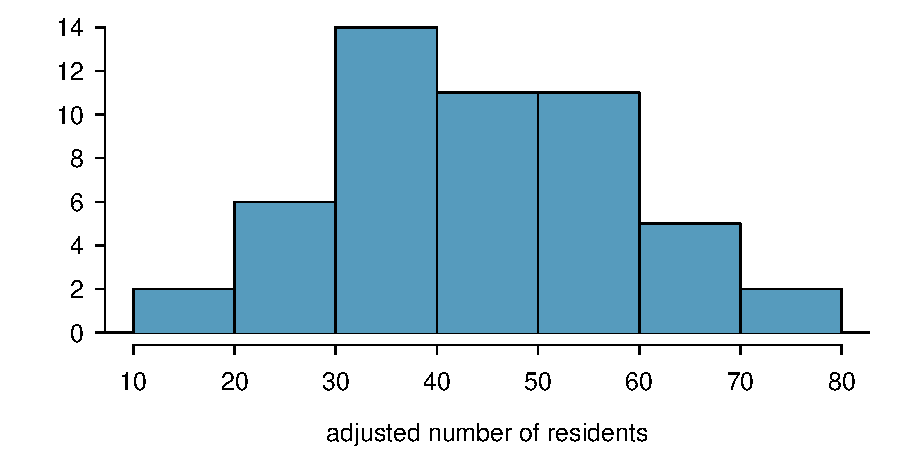
\includegraphics[width = \textwidth]{ch_intro_to_data_oi_biostat/figures/eoce/nursing_home/nursing_home_hist.pdf} 
\end{center}	
\end{minipage}
\begin{minipage}[c]{0.45\textwidth}
\begin{center}
	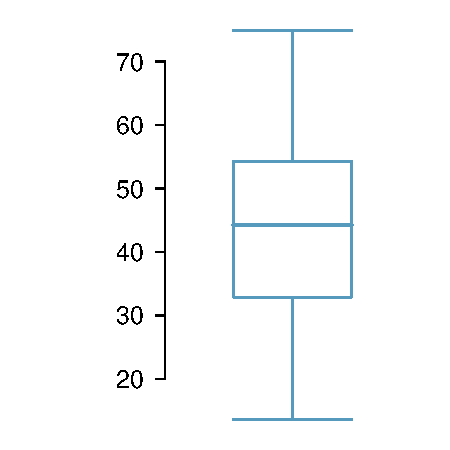
\includegraphics[width = \textwidth]{ch_intro_to_data_oi_biostat/figures/eoce/nursing_home/nursing_home_boxplot.pdf} 
\end{center}	
\end{minipage}
\begin{parts}
\item Is the distribution of adjusted number of nursing home residents symmetric or skewed? Are there any states that could be considered outliers?

\item Which plot is more informative: the histogram or the boxplot? Explain your answer.

\item What factors might influence the substantial amount of variability among different states? This question cannot be answered from the data; speculate using what you know about the demographics of the United States.
\end{parts}
}{}

% cite nursing home data, Pset 1, Q1


% 27 (oi_biostat)

\eoce{\qt{Eating disorders\label{korean_survey}}
In a 2003 survey examining weights and body image concerns among young Korean women, researchers administered a questionnaire to 264 female college students in Seoul, South Korea. The survey was designed to assess excessive concern with weight and dieting, consisting of questions such as "If I gain a pound, I worry that I will keep gaining." Questionnaires were given numerical scores on the Drive for Thinness Scale. Roughly speaking, a score of 15 is typical of Western women with eating disorders, but unusually high (90$^{th}$) percentile for other Western women. 

\begin{minipage}[c]{0.45\textwidth}
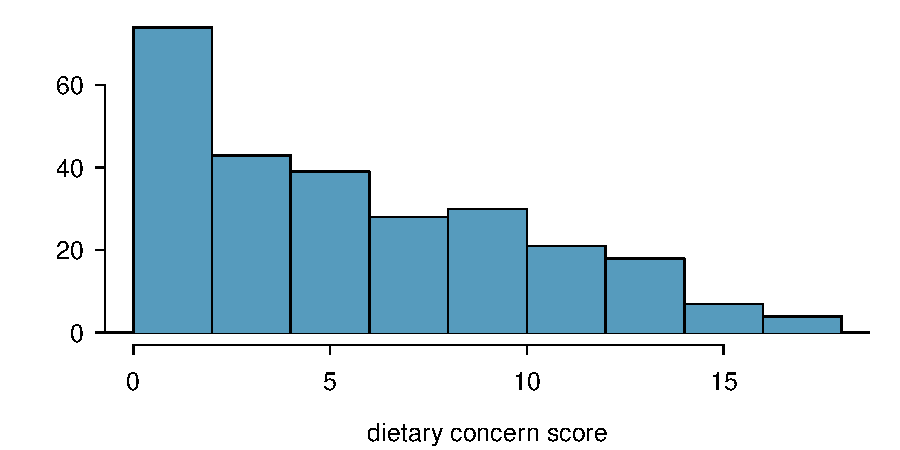
\includegraphics[width=\textwidth]{ch_intro_to_data_oi_biostat/figures/eoce/korean_survey/korean_survey_hist.pdf}
\end{minipage}
\begin{minipage}[c]{0.55\textwidth}
\begin{parts}
\item Describe the shape and spread of the scores for these Korean students.
\item Which measures of center and spread will provide a better summary of the data? 	
\end{parts}
\end{minipage}
}{}

% from problem 1.37, 7th ed Moore McCabe Craig, p. 25

% 28

\eoce{\qt{Midrange\label{midrange}} The \textit{midrange} of a distribution is defined as 
the average of the maximum and the minimum of that distribution. Is this statistic 
robust to outliers and extreme skew? Explain your reasoning.
}{}


%_______________
\subsection{Categorical data}


% 29

\eoce{\qt{Views on immigration\label{immigration}} 910 randomly sampled registered 
voters from Tampa, FL were asked if they thought workers who have illegally 
entered the US should be (i) allowed to keep their jobs and apply for 
US citizenship, (ii) allowed to keep their jobs as temporary guest workers 
but not allowed to apply for US citizenship, or (iii) lose their jobs and 
have to leave the country. The results of the survey by political ideology 
are shown below.\footfullcite{survey:immigFL:2012}
\begin{center}
\begin{tabular}{l l c c c c}
                        &                           & \multicolumn{3}{c}{\textit{Political ideology}} \\
\cline{3-5}
                        &                           & Conservative  & Moderate  & Liberal   & Total \\
\cline{2-6}
                        & (i) Apply for citizenship & 57            & 120       & 101       & 278 \\
                        & (ii) Guest worker         & 121           & 113       & 28        & 262 \\
\raisebox{1.5ex}[0pt]{\emph{Response}} & (iii) Leave the country    & 179       & 126       & 45        & 350 \\ 
                        & (iv) Not sure             & 15            & 4         & 1         & 20\\
\cline{2-6}
                        & Total                     & 372           & 363       & 175       & 910
\end{tabular}
\end{center}
\begin{parts}
\item What percent of these Tampa, FL voters identify themselves as conservatives?
\item What percent of these Tampa, FL voters are in favor of the citizenship option?
\item What percent of these Tampa, FL voters identify themselves as conservatives 
and are in favor of the citizenship option?
\item What percent of these Tampa, FL voters who identify themselves as 
conservatives are also in favor of the citizenship option? What percent of 
moderates share this view? What percent of liberals share this view?
\end{parts}
}{}

% 30 (oi_biostat)

\eoce{\qt{Flossing habits\label{flossing_habits}} Suppose that an anonymous questionnaire is given to patients at a dentist's office once they arrive for an appointment. One of the questions asks "How often do you floss?", and four answer options are provided: a) at least twice a day, b) at least once a day, c) a few times a week, and d) a few times a month. At the end of a week, the answers are tabulated: 31 individuals chose answer a), 55 chose b), 39 chose c), and 12 chose d). 
\begin{parts}
	\item Describe how these data could be numerically and graphically summarized.
	\item Assess whether the results of this survey can be generalized to provide information about flossing habits in the general population. 
\end{parts}
	
}{}

%_______________
\subsection{Relationships between two variables}

% 31, edited

\eoce{\qt{Mammal life spans\label{mammal_life_spans}} Data were collected on life spans (in 
	years) and gestation lengths (in days) for 62 mammals. A scatterplot of life span versus 
	length of gestation is shown below. \footfullcite{Allison+Cicchetti:1975}
	
	\noindent\begin{minipage}[c]{0.44\textwidth}
		\begin{parts}
			\item Does there seem to be an association between length of gestation and life span? If so, what type of association? Explain your reasoning.
			\item What type of an association would you expect to see if the axes of the plot were reversed, i.e. if we plotted length of gestation versus life span?
		\end{parts}\vspace{6mm}
	\end{minipage}
	\begin{minipage}[c]{0.55\textwidth}
		\begin{center}
			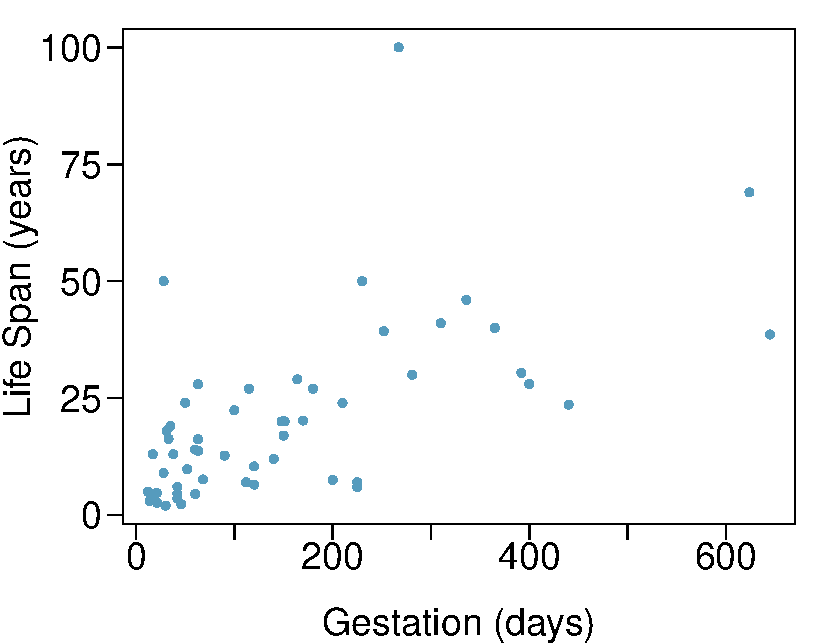
\includegraphics[width = 0.86\textwidth]{ch_intro_to_data_oi_biostat/figures/eoce/mammal_life_spans/mammal_life_spans_scatterplot.pdf}
		\end{center}
	\end{minipage}
}{}

\newpage

% 32

\eoce{\qt{Associations\label{association_plots}} Indicate which of the plots show a \\[1mm]
	\noindent\begin{minipage}[b]{0.35\textwidth}
		\begin{parts}
			\item positive association
			\item negative association
			\item no association
		\end{parts}
		Also determine if the positive and negative associations are linear or nonlinear. Each 
		part may refer to more than one plot. \vspace{30mm}
	\end{minipage}
	\begin{minipage}[b]{0.62\textwidth}
		\hfill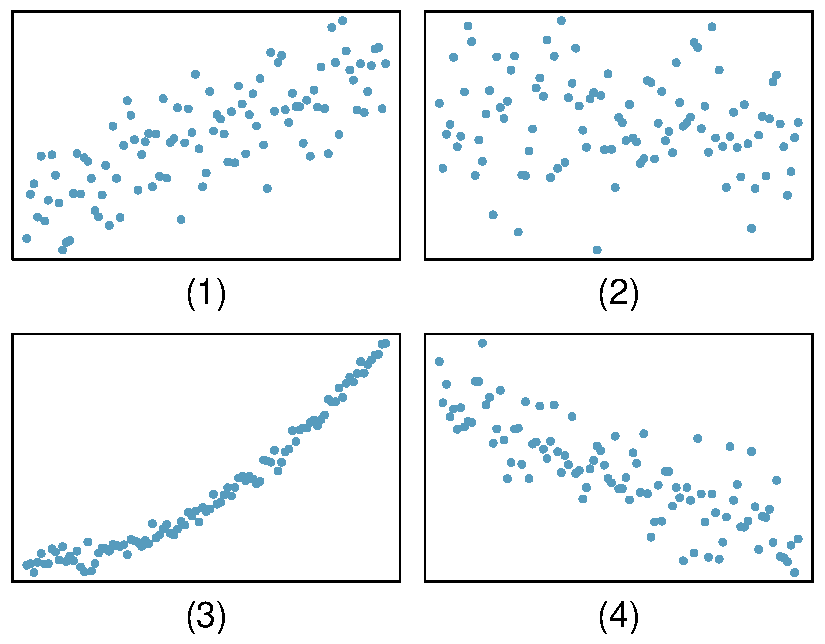
\includegraphics[width = 0.95\textwidth]{ch_intro_to_data_oi_biostat/figures/eoce/association_plots/association_plots.pdf}
	\end{minipage}
}{}

% 33 (oi_biostat)

\eoce{\qt{Adolescent fertility\label{adol_fertility}}
	Data are available on the number of children born to women aged 15-19 from 189 countries in the world for the years 1997, 2000, 2002, 2005, and 2006. The data are defined using a scaling similar to that used for the nursing home data in Exercise~\ref{nursing_homes}. The values for the annual adolescent fertility rates represent the number of live births among women aged 15-19 per 1,000 female members of the population of that age.
	
	\begin{center}
		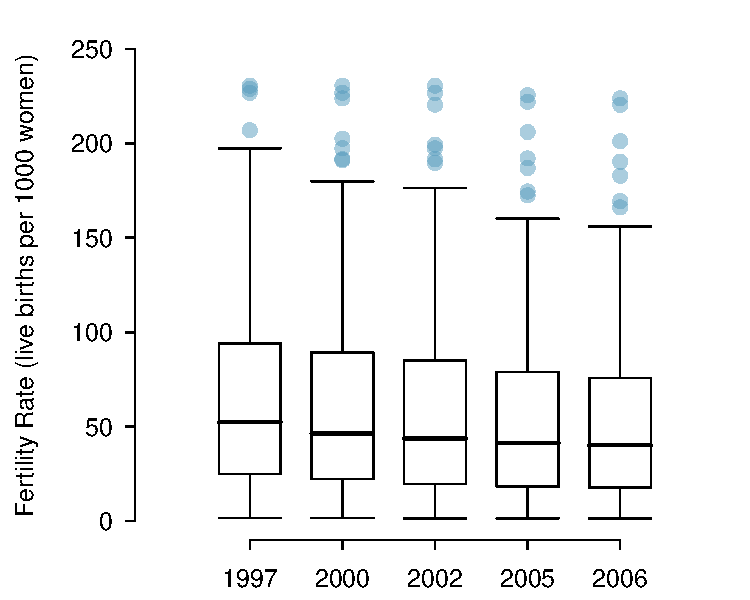
\includegraphics[width=0.7\textwidth]{ch_intro_to_data_oi_biostat/figures/eoce/adolescent_fertility/adol_fertility_boxplot.pdf}
	\end{center}
	
	\begin{parts}
		\item In 2006, the standard deviation of the distribution of adolescent fertility is 75.73. Write a sentence explaining the 75$^{th}$ percentile in the context of this data.
		\item For the years 2000-2006, data are not available for Iraq. Why might those observations be missing? Would the five-number summary have been affected very much if the values had been available?
		\item From the side-by-side boxplots shown above, describe how the distribution of fertility rates changes over time. Is there a trend?
	\end{parts}	
}{}

% 34 (oi_biostat)

\eoce{\qt{Smoking and stenosis\label{smoking_and_stenosis_intro}}
	Researchers collected data from an observational study to investigate the association between smoking status and the presence of aortic stenosis, a narrowing of the aorta that impedes blood flow to the body.
	\begin{center}
		\begin{tabular}{ll  cc c} 
			&			& \multicolumn{2}{c}{\textit{Smoking Status}} \\
			\cline{3-4}
			&			& Non-smoker 	& Smoker	& Total	\\
			\cline{2-5}
			& Absent & 67	& 54	& 121 \\
			\raisebox{1.5ex}[0pt]{\emph{Disease Status}}	& Present	& 43	& 51 	& 94 \\
			\cline{2-5}
			& Total		& 110	& 105	& 215
		\end{tabular}
	\end{center}
	\begin{parts}
		\item What percentage of the 215 participants were both smokers and had aortic stenosis? This percentage is one component of the \textit{joint distribution} of smoking and stenosis; what are the other three numbers of the joint distribution?
		\item Among the smokers, what proportion have aortic stenosis? This number is a component of the conditional distribution of stenosis for the two categories of smokers. What proportion of non-smokers have aortic stenosis?
		\item In this context, relative risk is the ratio of the proportion of smokers with stenosis to the proportion of non-smokers with stenosis. Relative risks greater than 1 indicate that smokers are at a higher risk for aortic stenosis than non-smokers; relative risks of 1.2 or higher are generally considered cause for alarm. Calculate the relative risk for the 215 participants, comparing smokers to non-smokers. Does there seem to be evidence that smoking is associated with an increased probability of stenosis?
	\end{parts}
}{}

% citation: stenosis data

% 35 (oi_biostat)

\eoce{\qt{Anger and cardiovascular health\label{anger_chd}}
	Trait anger is defined as a relatively stable personality trait that is manifested in the frequency, intensity, and duration of feelings associated with anger. People with high trait anger have rage and fury more often, more intensely, and with long-laster episodes than people with low trait anger. It is thought that people with high trait anger might be particularly susceptible to coronary heart disease; 12,986 participants were recruited for a study examining this hypothesis. Participants were followed for five years. The following table shows data for the participants identified as having normal blood pressure (normotensives).
	
	\begin{center}
		\begin{tabular}{l l c c c c}
			&                           & \multicolumn{3}{c}{\textit{Trait Anger Score}} \\
			\cline{3-5}
			&                           & Low  & Moderate  & High   & Total \\
			\cline{2-6}
			& Yes & 53            & 110     & 27       & 190 \\
			\raisebox{1.5ex}[0pt]{\emph{CHD Event}} & No    & 3057       & 4704      & 606       & 8284 \\ 
			& Total                     & 3110           & 4731     & 633      & 8474
		\end{tabular}
	\end{center}
	
	\begin{parts}
		\item What percentage of participants have moderate anger scores?
		\item What percentage of individuals who experienced a CHD event have moderate anger scores?
		\item What percentage of participants with high trait anger scores experienced a CHD event (i.e., heart attack)?
		\item What percentage of participants with low trait anger scores experienced a CHD event?
		\item Are individuals with high trait anger more likely to experience a CHD event than individuals with low trait anger? Calculate the relative risk of a CHD event for individuals with high trait anger compared to low trait anger.
		\item Researchers also collected data on various participant traits, such as level of blood cholesterol (measured in mg/dL). What graphical summary might be useful for examining how blood cholesterol level differs between anger groups?
	\end{parts}
}{}

% cite anger_chd paper


%_______________
\subsection{Exploratory data analysis}

Since exploratory data analysis relies heavily on the use of computation, refer to the companion text for exercises related to this section.